\chapter{Test lab}
\label{app:network}
\emph{This appendix describes and visualizes the test lab that was used to perform the tests.}

\section{General description}

In order to perform the required tests, a test lab is of course needed. The lab is an expansion of a production environment used in a Small Office Home Office (SOHO). The existing hardware equipment consists of a Belgacom router, a central switch, a physical tower server running the Xen hypervisor and some connections leading to the clients, other switches and network printers. Figure \ref{fig:network} provides the reader with a visual representation of the network.

This network has been expanded with a 1U rack server and another tower server. On the 1U rack server and the tower server, Microsoft Windows Server 2012 R2 was installed as well as the Hyper-V role. So both servers run the Hyper-V hypervisor. In fact, due to \citep{Best1} and \citep{Best2}, it is recommended not to install any other roles besides the Hyper-V role. This is because the hypervisor partition is placed in between the parent partition and the hardware. Also, it will keep the management system (the Hyper-V host) clean as no updates are required but for the Hyper-V role.\\ \\
Thus there exist three virtual networks: a Xen - based virtual network and two Hyper-V based networks. The reason for combining two different virtual networks is that prior to starting this master thesis, I had quite a lot of experience with the Xen hypervisor, but almost none with Microsoft's counterpart.

Another reason for the mixed environment is that I wanted to check whether the two different virtual networks are able to cooperate with each other as they should.

\section{Technical description}

\subsection{Hardware overview}

SSH is used to remotely access the virtual machines running on the Xen hypervisor, wheras Remote Desktop Connection (RDP) is used to connect to the Hyper-V hypervisor as well as to access the dual-boot server.

Since only one external IP address is available, different ports were used for RDP, ranging from 3389 to 3395. \\
The Xen host, the first Hyper-V host and second Hyper-V host run 4, 5 and 3 VM's, respectively. \\
Below is a table specifying the hardware of the different servers used in the test lab.

\begin{table}[h]
\begin{tabular}{|l|l|l|l|}
\hline
System                  & Xen server                & Hyper-V server             & Dual-boot server \\ \hline
Processor brand         & AMD                       & Intel                      & Intel            \\ \hline
Processor type          & Athlon II x2 240e & Core 2 Quad Q9550 & Core i7 930    \\ \hline
Core speed	&	2.8 GHz	&	2.83 GHz 	&	2.80 GHz \\ \hline
Number of cores         & 2                         & 4                          & 4                \\ \hline
Number of sockets    & 1                         & 1                          & 1                \\ \hline
Number of virtual cores & 2                         & 4                          & 8                \\ \hline
Memory amount and type  & 8 GB DDR3                 & 8 GB DDR2                  & 8 / 16 GB DDR3       \\ \hline
\# Harddisk drives      & 4                         & 4                          &    3              \\ \hline
RAID type               & LVM                       & 5                          & 5                \\ \hline
Hardware RAID?          & NO                        & YES                        & YES              \\ \hline
Ethernet speed          & 1 Gbps                    & 1 Gbps                    & 1 Gpbs          \\ \hline
\end{tabular}
\caption{Overview of the hardware used in the test lab}
\end{table}

\subsection{Networking overview}
The table below provides an overview of the IP addressing scheme.
\begin{table}[h!]
\begin{tabular}{|l|l|}
\hline
\textbf{Device}                 & \textbf{IP address} \\ \hline
Belgacom router                 & 192.168.1.1         \\ \hline
Xen host                      & 192.168.1.2         \\ \hline
Hyper-V host 1 (management)     & 192.168.1.7         \\ \hline
Hyper-V host 1 (external switch) & 192.168.1.6         \\ \hline
Hyper-V host 2 (external switch) & 192.168.1.8	\\ \hline
Hyper-V VM 1                    & 192.168.1.50        \\ \hline
Hyper-V VM 2                    & 192.168.1.51        \\ \hline
Hyper-V VM 3			& 192.168.1.12 \\ \hline
Hyper-V domain controller VM	&	192.168.1.150 \\ \hline
Hyper-V backup domain controller VM	&	192.168.1.152\\ \hline
Hyper-V Virtual Machine Manager VM	&	192.168.1.151 \\ \hline
Hyper-V Windows Azure Pack VM &	192.168.1.160\\ \hline
Xen VM 1                        & 192.168.1.11        \\ \hline
Xen VM 2                        & 192.168.1.14        \\ \hline
Xen VM 3                        & 192.168.1.16        \\ \hline
\end{tabular}
\end{table}

\section{Visualization of the test lab}

\noindent\begin{minipage}{\textwidth}
    \centering
    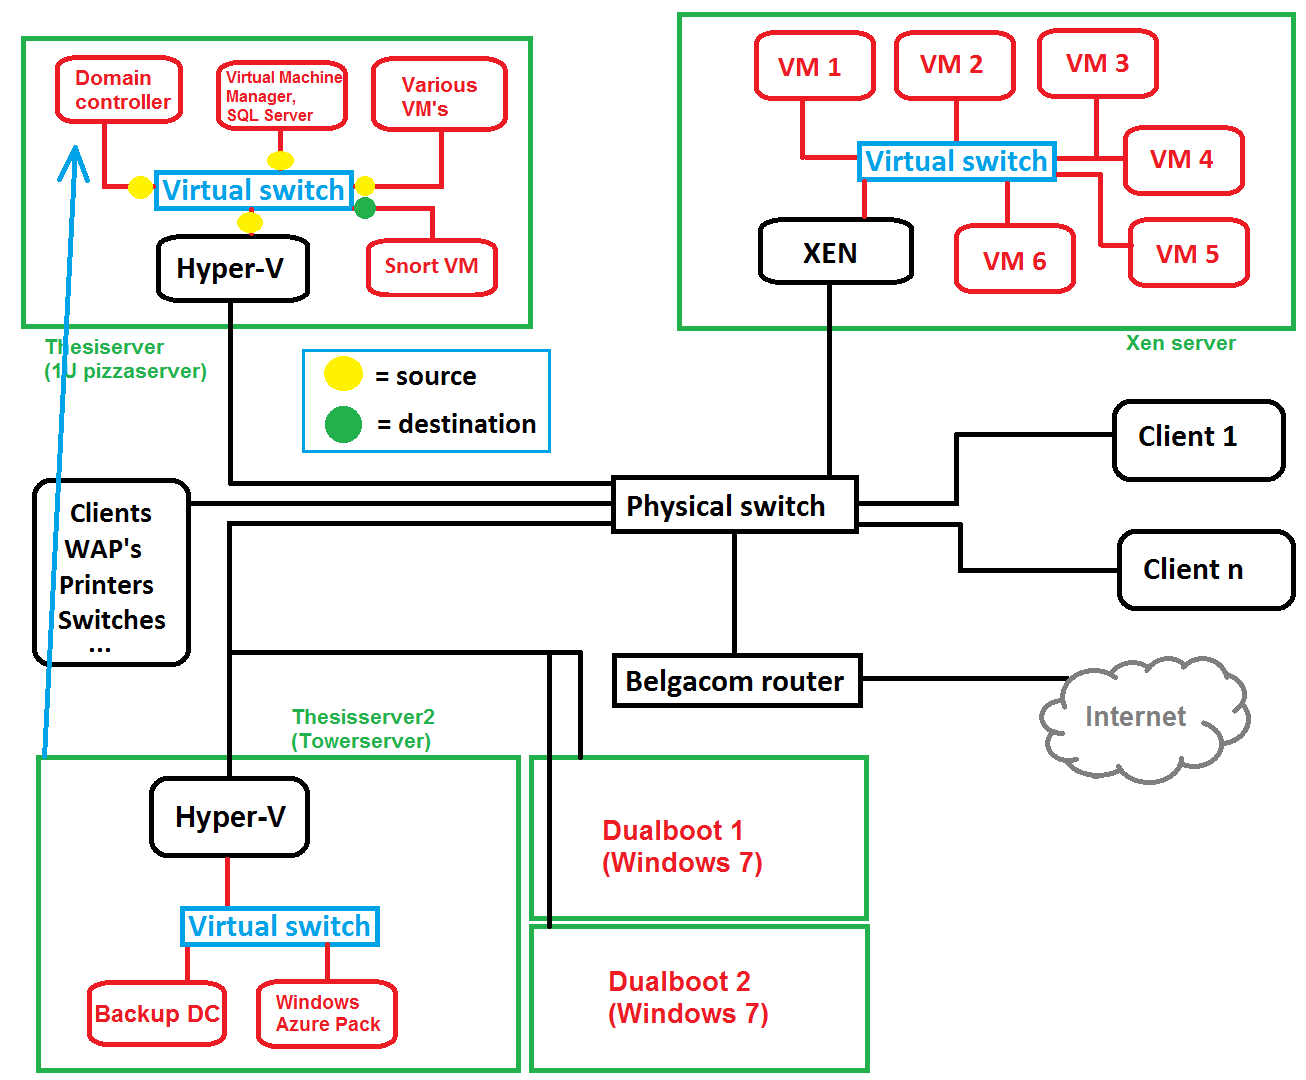
\includegraphics[angle=270,scale=0.57]{Network.png}
    \captionof{figure}{The network setup}
\label{fig:network}
\end{minipage}